
\section{The Planner}

The first big decision we faced during the development of PokerShark was choosing which planner we wanted to use. We had several requirements that we wanted present in the planner. First, the planner must be performant. We are not looking to find the most efficient planner because we anticipate that the network size will be limited to a few hundred tasks. We prefer the planner to be battle-tested. Many planners were conceived and developed in academic settings but have yet to be tested in the real world. We wanted to avoid these planners. Poker is a complex domain, and a game of poker has many elements and variables, making it more challenging to describe the game's state. That is why we need the planner to have an expressive description language that is easy to use and not too difficult to learn. Furthermore, defining the bot strategy will be tedious and require a lot of fine-tuning. Hence the planner needs to provide easy debugging tools.

Typically HTN planners do not support utility nur expected utility, which is essential to our work. We have to assume that we will have to extend the functionality of the planner, so we have to consider the extensibility of the planner, which introduces an array of factors, such as the programming language, the quality of the code, the architecture, the frameworks..., and a lot of other factors. Most likely, we will also have to modify the description language, which makes the parser of the planner a very important factor to consider. Lastly, we have to think about the integration between the planner and the bot. We prefer a seamless integration where the bot can notify the planner about the game's state and receive the planner's decision. We will explore next some of the planners that we have considered:



\subsection*{JSHOP}

JSHOP is part of the SHOP (Simple Hierarchical Ordered Planner) project\footnote{\url{http://www.cs.umd.edu/projects/shop/description.html}} developed by the University of Maryland. The planner is a Java-based implementation of SHOP2. JSHOP was first released in 2005, making it one of the older planners we have considered. It was part of numerous studies and was used in many applications, which makes us more confident in its performance and reliability. SHOP planners have a custom description format developed and extended throughout the years. JSHOP uses ANTLR3\footnote{\url{https://www.antlr3.org/}} to parse domain and problem definitions. Rather than interpreting the definition files, JSHOP compiles them into Java code that the planner can call, which makes JSHOP harder to integrate.

\begin{figure}[h]
    \centering
    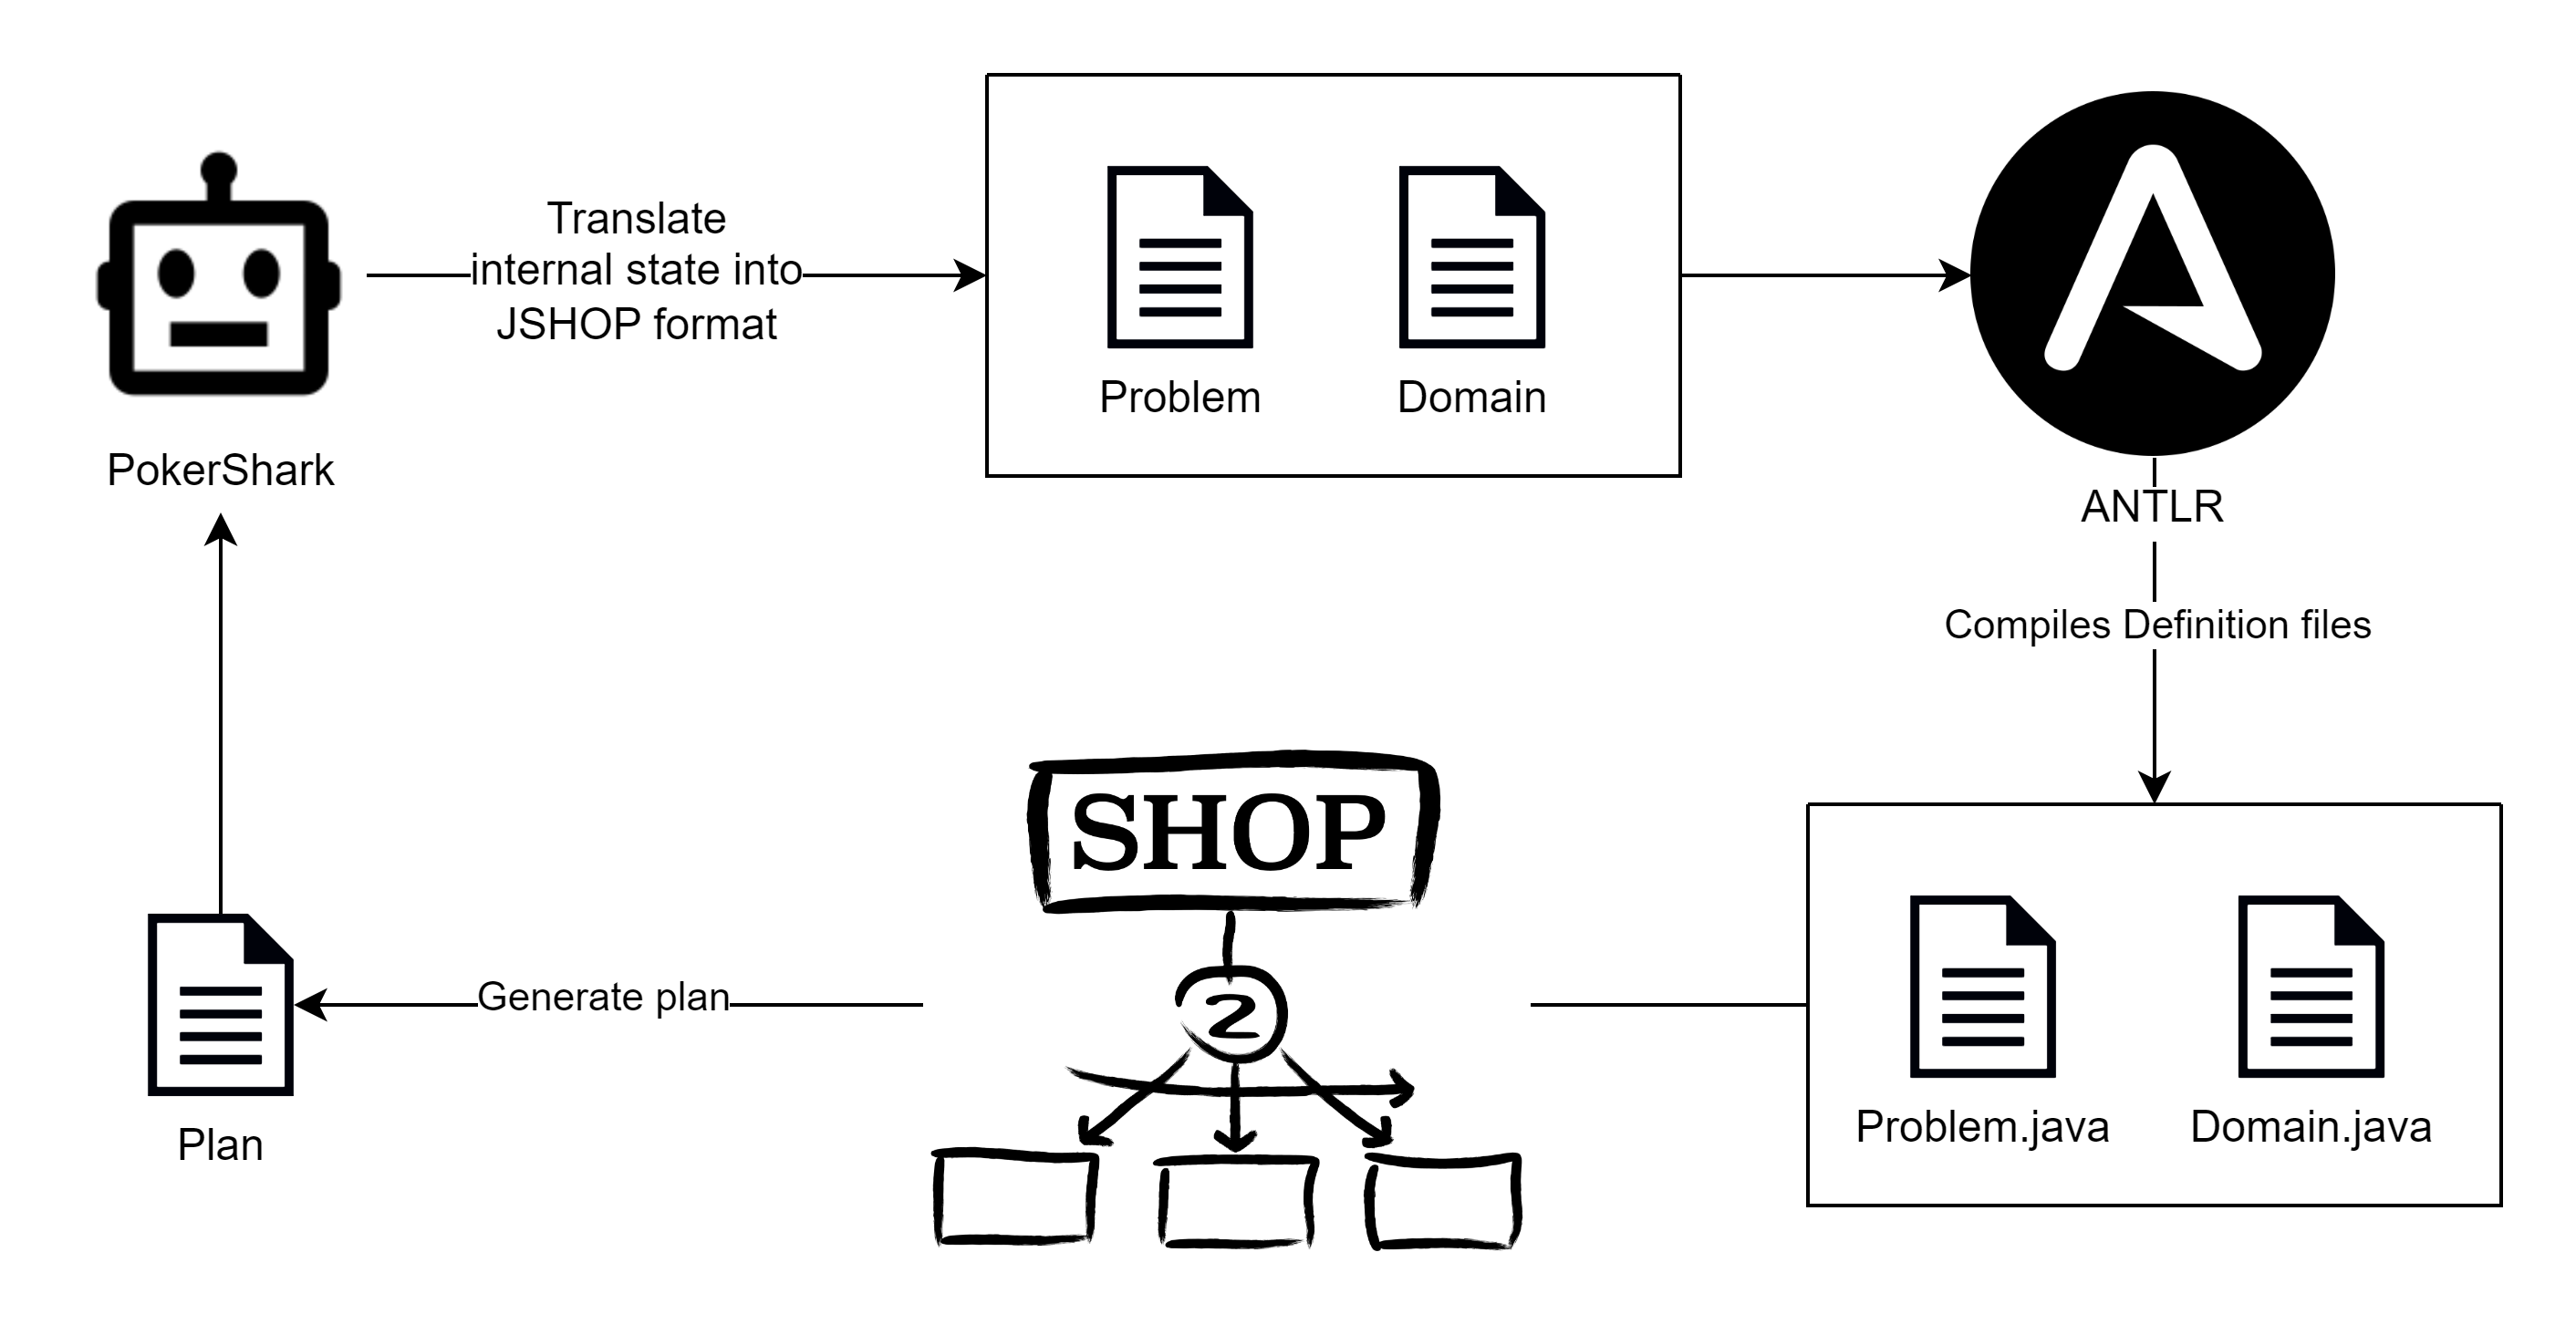
\includegraphics[width=\textwidth]{graphics/jshop.png}
    \caption{Multiple translation and read/write operations required.}
    \label{fig:jshop}
\end{figure}



JSHOP does not support utility nur expected utility. Although the code is well-documented and can be considered clean, it will be challenging to extend due to the architecture. Since the description format also needs to be extended, ANTLR rules and grammar files must be modified. ANTLR3 is notoriously tedious, and we rather not deal with it. The planner has a GUI to run plans, which can be helpful for debugging, but it is not ideal. Nevertheless, JSHOP is a great planner with some advantages and disadvantages that must be considered for the final decision.





\subsection*{SHOP3}
SHOP3\footnote{\url{https://shop-planner.github.io/}} is the successor of SHOP2, which means it benefits from all the expertise that went into SHOP2. Unfortunately, it is Lisp-based, which is personally a big downside. In addition, the planner does not support expected utility and must be extended. On the other hand, the planner supports PDDL and provides excellent debugging features.



\subsection*{PANDA}

The PANDA framework\footnote{\url{https://panda-planner-dev.github.io/}} is one of the most promising candidates. The planner is developed and maintained by the Institute of Artificial Intelligence at Ulm University. The PANDA framework consists of several c++ modules that provide various features, such as plan verification and repair. However, the planner uses a custom parser that supports HDDL and the SHOP format. Modifying a custom parser can take a lot of work, especially with the planner's complex parsing pipeline that involves many modules and transitionary formats. Undoubtedly, PANDA is a good planner but has yet to be battle-tested, and it does not have great potential for extension.



\subsection*{InductorHtn}

InductorHtn\footnote{\url{https://github.com/EricZinda/InductorHtn}} was not developed in an academic setting. It was originally intended to be part of an ios-based game engine. The planner draws a lot of inspiration from SHOP2. It uses Prolog as a description format, but it also provides the ability to use native C++ constructs to define the planning domain and problem. This is a significant advantage as no compilation is required to run the planner, which greatly facilitates the integration process. InductorHtn also provides good debugging features. However, the planner's code lacks documentation and does not look like a great candidate for modification.


\subsection*{FluidHTN}

FluidHTN\footnote{\url{https://github.com/ptrefall/fluid-hierarchical-task-network}} is a feature-rich planner based around the Builder pattern's principles. The planner offers numerous features, including partial planning, domain splicing, and early rejection. FluidHTN supports only native domain definition. However, it has a powerful and expressive domain builder, which greatly simplifies domain and problem description. Moreover, it has great debugging tools that are superior to almost all other planners.

FluidHTN is the first candidate that was built with extensibility in mind. As a result, all the planner's components and elements are easy to modify, extend or replace. In addition, the planner has surprisingly a big active community, especially game developers, which suggests that the planner is performant and battle-tested enough for us to consider a good candidate. Finally, having native domain definition support makes the integration much easier. 


\begin{table}[H]
    \centering
    \footnotesize
    \begin{tabular}{|l|c|c|c|c|c|l|}
        \hline
        \textbf{Planner}     & \textbf{Maturity} & \textbf{Expressivnise} & \textbf{Extensibility} & \textbf{Debugging} & \textbf{Integration} & \textbf{Overall} \\ \hline
        \textbf{JSHOP}       & 5                 & 4                      & 3                      & 2                  & 2                    & \Stars{3.2}      \\ \hline
        \textbf{SHOP3}       & 5                 & 4                      & 1                      & 3                  & 1                    & \Stars{2.8}      \\ \hline
        \textbf{PANDA}       & 2                 & 4                      & 1                      & 2                  & 0                    & \Stars{1.8}      \\ \hline
        \textbf{InductorHtn} & 4                 & 5                      & 3                      & 3                  & 2                    & \Stars{3.4}      \\ \hline
        \textbf{FluidHTN}    & 5                 & 5                      & 5                      & 4                  & 5                    & \Stars{4.8}      \\ \hline
    \end{tabular}
    \caption{Planner comparison.}
    \label{tab:planner-comparison}
\end{table}

Table \ref{tab:planner-comparison} shows our final evaluation of the planners. We have used a 5-point scale to evaluate the planners. Our evaluation is based on the following criteria: maturity, expressiveness, extensibility, debugging, and integration and is heavily influenced by our preferences. Overall, FluidHTN is the most complete planner for our use case. 

\subsubsection*{FluidHTN Showcase}

FluidHTN is clearly influenced by game development but is also designed to be adaptable for any use case. The planner has a unique structure. Thus we would like to dedicate this section to showcasing its underlying concepts. FluidHTN is built for an agent to be dynamic. That is why it does not use problem definitions but instead uses the concept of world state, which is a model of the agent's environment. Programmatically, the state of the world is a simple array of objects. The world state may be shared with other actors or used as a model in isolation. Combining a shared state with operators that can affect the state turns the planner into a complete agent, which the planner excels at, especially with its state tracking, plan verification, and replanning.

\begin{figure}[h]
    \centering
    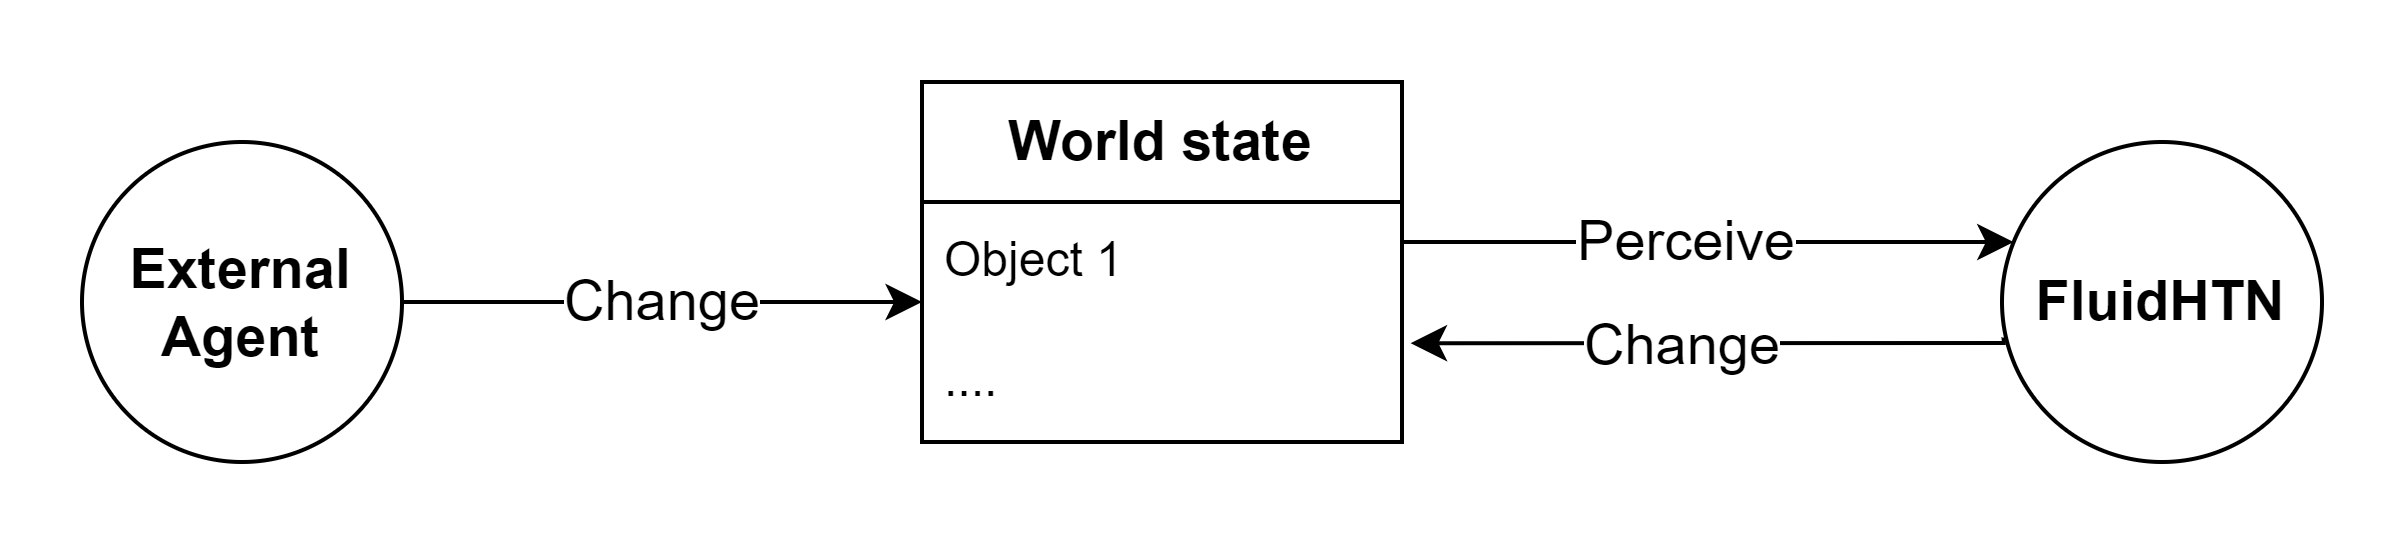
\includegraphics[width=\textwidth]{graphics/agent_3.png}
    \caption{FluidHTN with shared state.}
    \label{fig:agent}
\end{figure}

Using the planner in this configuration has numerous advantages, but it forces the planning domain to be static. We would like to have more control over the planning domain. Therefore we are not going to use the planner in this configuration. Instead, we will use the planner as a standalone planner that is not aware of the agent's state. This configuration is also useful for debugging and testing purposes. Instead, we will use FluidHTN as a standalone planner that receives the planning domain and context from the bot.

\begin{figure}[h]
    \centering
    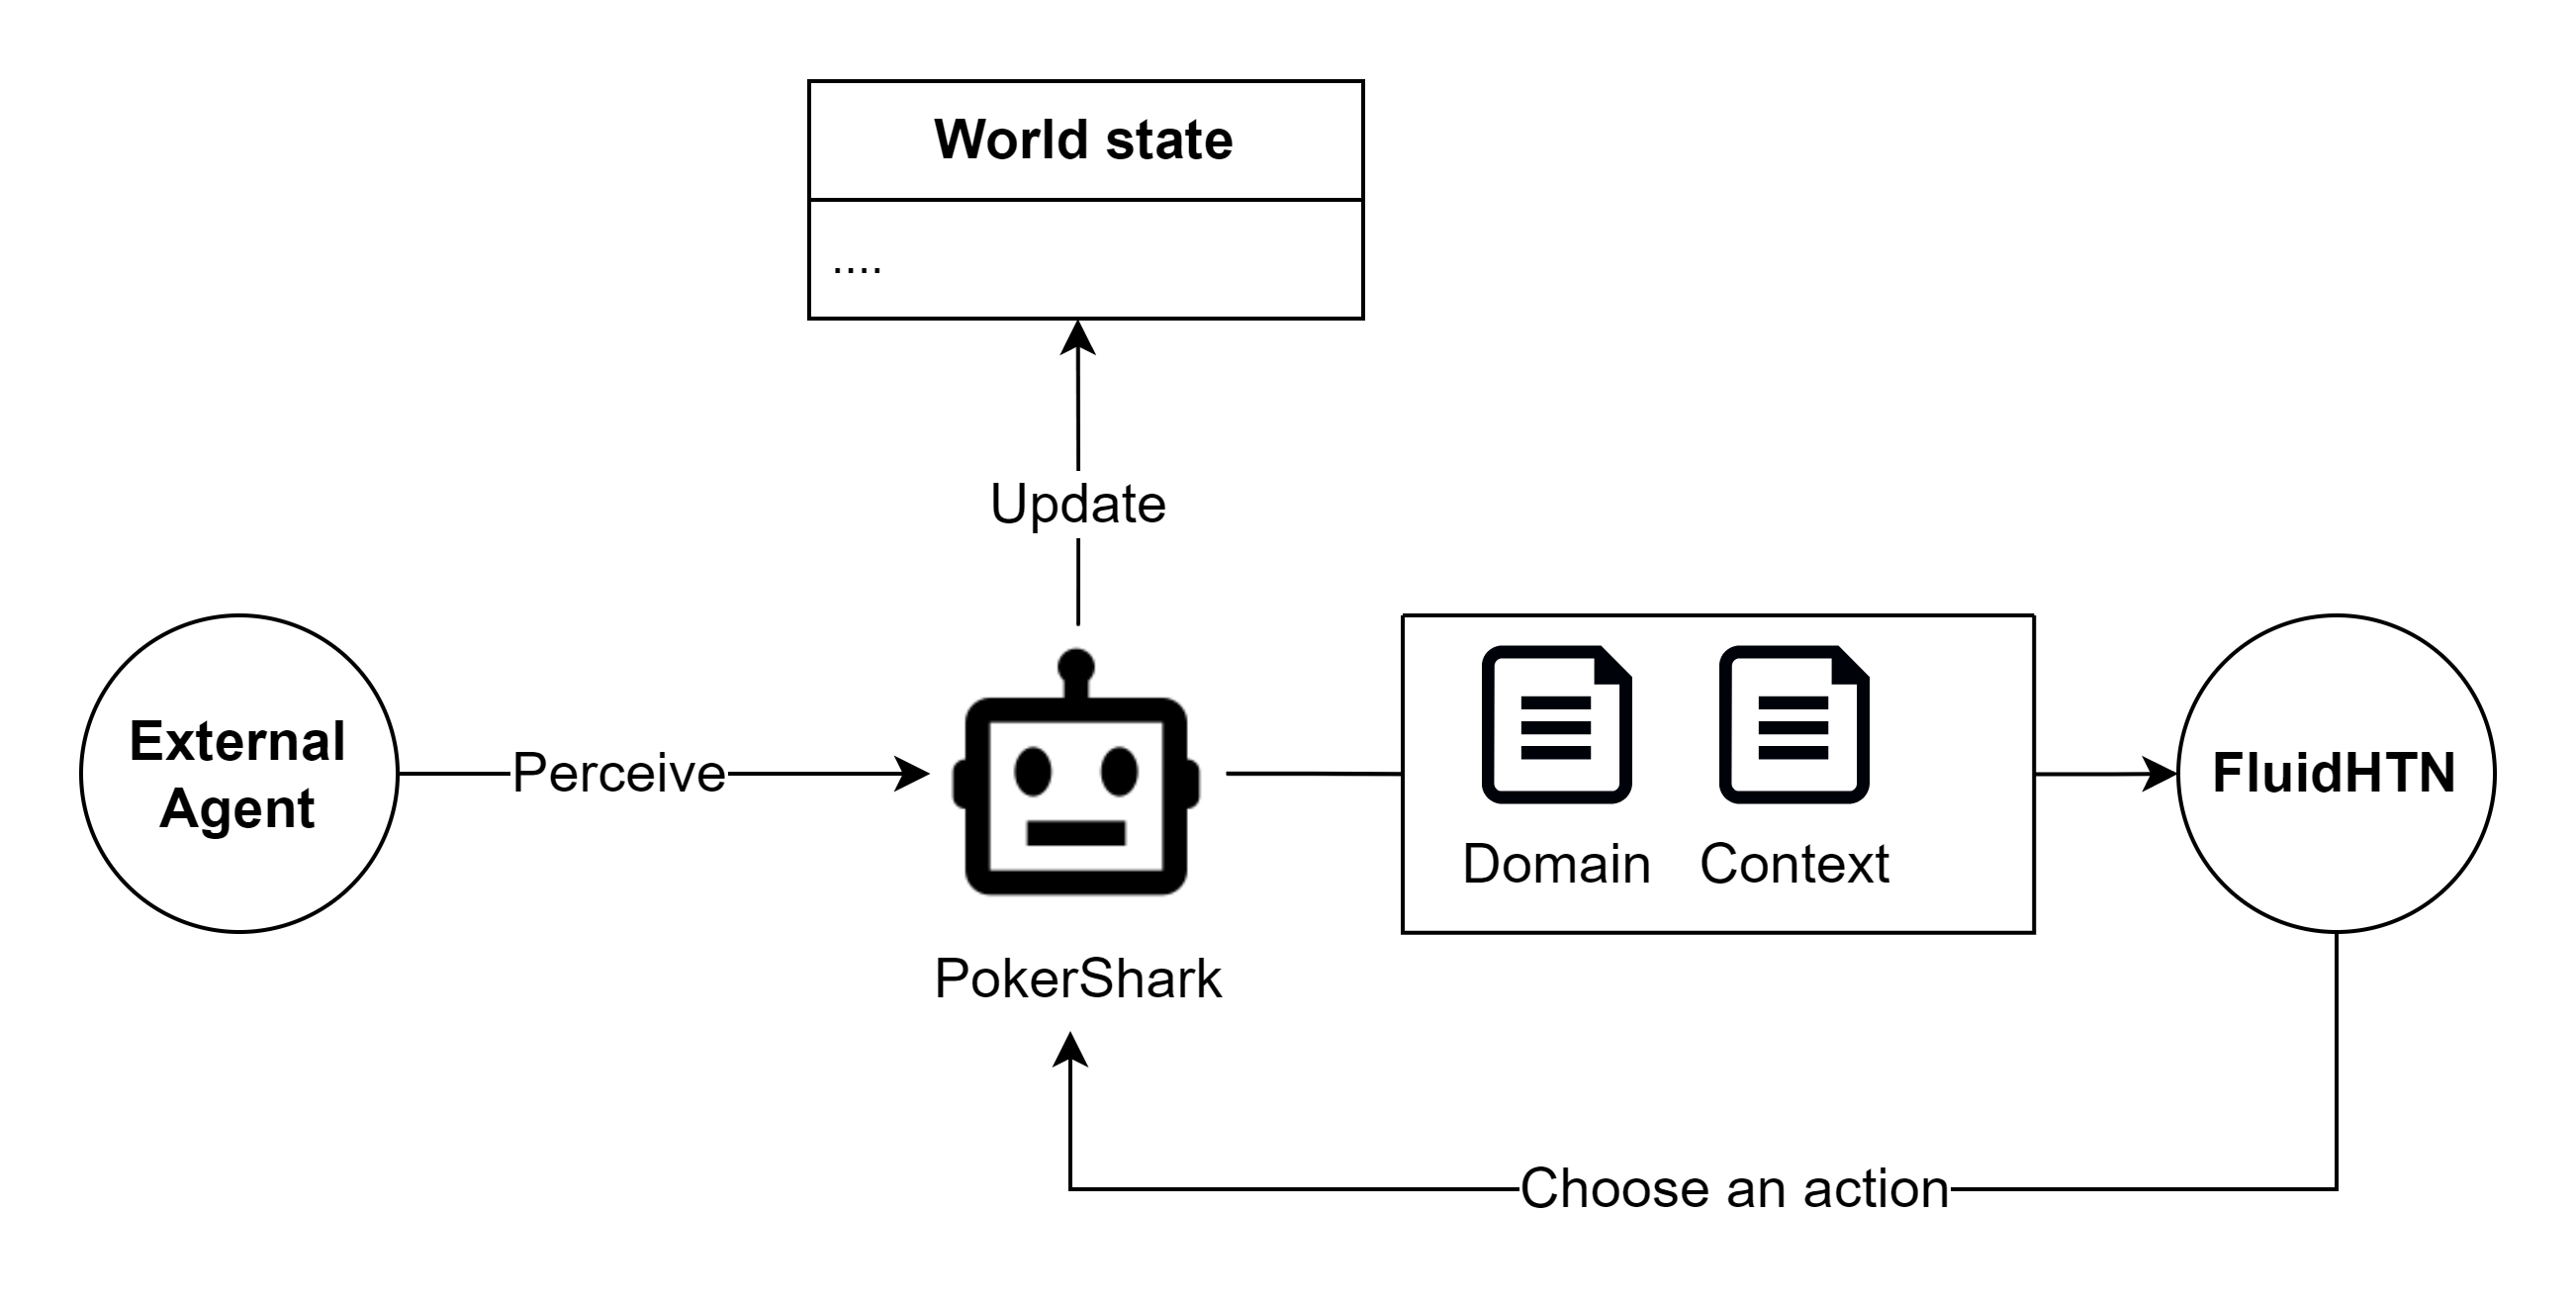
\includegraphics[width=\textwidth]{graphics/structure.png}
    \caption{PokerShark architecture.}
    \label{fig:PokerSharkArchitecture}
\end{figure}

FluidHTN adopts the concepts of compound and primitive tasks of HTN. Compound tasks can be implemented using one of two structures. The first structure is called \textit{Sequence}. In order to decompose a Sequence, all of its sub-tasks must decompose successfully in contrast to the second structure, the \textit{Select}, which only requires the decomposition of one sub-task to be successfully decomposed. It should be noted that preconditions can be applied to tasks regardless of type.


\begin{figure}[h]
    \centering
    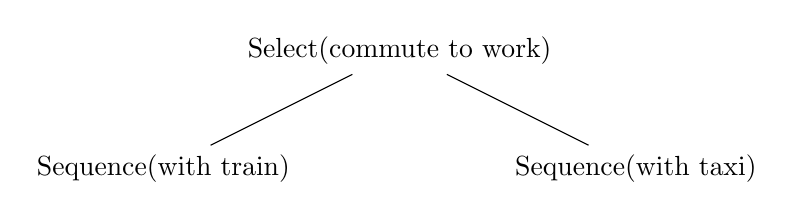
\begin{tikzpicture}
        \node {Select(commute to work)} [sibling distance = 6cm]
            child { 
                node{Sequence(with train)} 
                }
            child {
                node{Sequence(with taxi)}
                };
    \end{tikzpicture}
    \caption{Selects can choose one path, whereas Sequences need to decompose all subtasks.}
    \label{fig:select_sequence}
\end{figure}

The architecture of the planner makes it easy to introduce new representations of any component in the planning process. For example, Listing \ref{lst:RandomSelector} shows RandomSelector, which randomly selects and decomposes one of its subtasks.

\begin{Listing}
    \begin{lstlisting}[language={[Sharp]C}]
    public class RandomSelector : Selector
    {
        protected DecompositionStatus OnDecompose(IContext c, int i, out Queue<ITask> result)
        {
            var taskIndex = new Random().Next(i, Subtasks.Count);
            var task = Subtasks[taskIndex];
            return OnDecomposeTask(c, task, taskIndex, null, out result);
        }
    }
    \end{lstlisting}
    \caption{RandomSelector definition.}
    \label{lst:RandomSelector}
\end{Listing}

Primitive tasks are defined as actions where each action could have a set of preconditions and a set of effects. FluidHTN has three effect types: PlanOnly, PlanAndExecute, and Permanent. Because of the architecture that we are using, it does not matter what type of effect our operators have because our world state is updated by the bot, not the planner. Lastly, FluidHTN provides great readability if used probably. Listing \ref{lst:readability} shows a snippet of PokerShark domain builder.
\begin{Listing}
    \begin{lstlisting}[language={[Sharp]C}]
        Select("Raise Recommendation");    
            IfRaiseRecommendation();
            Select("Too Risky Raise");
                IfRaiseRecommendationTooRisky();
                Action("Fold if call to risky");
                    IfCallTooRisky();
                    Do(Fold);
                End();
            End();
        ...
    \end{lstlisting}
    \caption{Snippet of PokerShark domain builder.}
    \label{lst:readability}
\end{Listing}